% !TeX encoding = UTF-8

\documentclass[journal,twoside]{IEEEtran}

\usepackage{cite}

\ifCLASSINFOpdf
   \usepackage[pdftex]{graphicx}
  % declare the path(s) where your graphic files are
   \graphicspath{{./images/}}
  % and their extensions so you won't have to specify these with
  % every instance of \includegraphics
   \DeclareGraphicsExtensions{.pdf,.jpeg,.png}
\else
  % or other class option (dvipsone, dvipdf, if not using dvips). graphicx
  % will default to the driver specified in the system graphics.cfg if no
  % driver is specified.
  % \usepackage[dvips]{graphicx}
  % declare the path(s) where your graphic files are
  % \graphicspath{{../eps/}}
  % and their extensions so you won't have to specify these with
  % every instance of \includegraphics
  % \DeclareGraphicsExtensions{.eps}
\fi
\usepackage[cmex10]{amsmath}
\allowdisplaybreaks
\usepackage{array}
\usepackage{url}
\hyphenation{op-tical net-works semi-conduc-tor}

% ***ADDED BY JONAS***
\usepackage{wrapfig}
\usepackage{url}
\usepackage{nohyperref}
%for columns spanning multiple rows in tables
\usepackage{multirow}
%use the booktabs package to get (much!) better vertical spacing above and below "rules" (horizontal lines), resulting in a much more professional look of your tables.
%use the colortbl package to add color to tables.
\usepackage{booktabs,colortbl}

\usepackage{setspace}
\setstretch{0.99}
\usepackage{amsfonts}
\renewcommand{\vec}[1]{\mathbf{#1}}
% ********************

\begin{document}
\title{Temporal Instanton Analysis:\\
Development and Implementation}
% author names and IEEE memberships
% note positions of commas and nonbreaking spaces ( ~ ) LaTeX will not break
% a structure at a ~ so this keeps an author's name from being broken across
% two lines.
% use \thanks{} to gain access to the first footnote area
% a separate \thanks must be used for each paragraph as LaTeX2e's \thanks
% was not built to handle multiple paragraphs

\author{Jonas~A.~Kersulis,~\IEEEmembership{Student~Member,~IEEE,}
        ... %and~Ian~A.~Hiskens,~\IEEEmembership{Fellow,~IEEE}% <-this % stops a space
\thanks{The authors are with the Department of Electrical Engineering and Computer Science, University of Michigan, Ann Arbor, MI 48104 USA (e-mail: 
kersulis@umich.edu; hiskens@umich.edu)}%
\thanks{This work was supported by the Los Alamos National Laboratory Grid Science Program, subcontract 270958.}}%
%\thanks{Manuscript received ____; revised __.}}

% The paper headers
\markboth{IEEE Transactions on Power Systems,~Vol.~--, No.~-, ---~201-}%
{Kersulis and Hiskens: Temporal Instanton Analysis}
% The only time the second header will appear is for the odd numbered pages
% after the title page when using the twoside option.
% 
% *** Note that you probably will NOT want to include the author's ***
% *** name in the headers of peer review papers.                   ***
% You can use \ifCLASSOPTIONpeerreview for conditional compilation here if
% you desire.

\maketitle

\begin{abstract}
A previously-developed method for studying a transmission network's vulnerability to wind forecast inaccuracy is expanded. The method uses optimization to find a likely wind generation pattern that brings a specified line to an unacceptably high temperature. The objective quantifies wind pattern likelihood in terms of distance from the forecast, respecting spatial and temporal correlation between wind sites and time intervals. The set of constraints enforces power balance and ensures a chosen line in the network reaches a fixed temperature by the final time step. The thermal constraint is second-order in voltage angle differences, and is based on a DC-approximate line loss formulation. Repeatedly solving the QCQP for all lines in the network yields a set of instanton candidate generation patterns, which may then be sorted by likelihood. Having described the temporal instanton QCQP and its solution, the paper turns to a discussion of implementation details. Finally, a series of numerical experiments is presented. These experiments demonstrate the effect of an instanton pattern on line temperature trajectory, the effects of wind covariance on instanton analysis, and algorithm scaling properties.
\end{abstract}

% Note that keywords are not normally used for peerreview papers.
\begin{IEEEkeywords}
forecast uncertainty, optimization, transmission operations, wind energy
\end{IEEEkeywords}

% For peer review papers, you can put extra information on the cover
% page as needed:
% \ifCLASSOPTIONpeerreview
% \begin{center} \bfseries EDICS Category: 3-BBND \end{center}
% \fi
%
% For peerreview papers, this IEEEtran command inserts a page break and
% creates the second title. It will be ignored for other modes.
\IEEEpeerreviewmaketitle

\section{Introduction}\label{sec:intro}
\IEEEPARstart{A}{wind} forecast error that was once inconsequential is now vexatious. As wind grows into a major transmission-scale energy source, system operators find themselves frequently dealing with wind-induced network congestion \cite{rogers2010}. Operators use wind forecast data to steer the network, but wind forecasts are significantly less accurate than generation and demand predictions \cite{parsons2004}. Might forecast deviations compound across a collection of wind farms to overheat a transmission line? Which lines are most vulnerable to such an event? Temporal instanton analysis addresses these questions by identifying sag-inducing wind patterns and ranking them according to likelihood. The intersection of likely wind patterns with those that cause excessive line heating is of interest to system operators and planners, who may use this information to better prepare for renewable generation uncertainty.

Instanton analysis belongs to the family of distance to failure algorithms. It was introduced in \cite{chertkov2011} and \cite{chertkov2011a}, where the DC power flow approximation was used to represent a network's feasible operating region as a set of linear constraints. These constraints form the faces of a high-dimensional polytope that contains all feasible network states. Distance to failure is intuitively understood to be the shortest distance between an operating point and the surface of the constraint polytope. As shown in \cite{chertkov2011a}, one can use convex optimization to quickly find the smallest shift in wind generation that will drive the network to a chosen polytope face. Once every face has been considered, the collection of shifts may be sorted by distance from the forecast operating point. The wind pattern corresponding to the shortest distance between the forecast operating point and the boundary of the constraint polytope is termed the instanton; it is the smallest shift in wind generation that will drive the network to the brink of infeasibility.

\begin{figure}
\centering
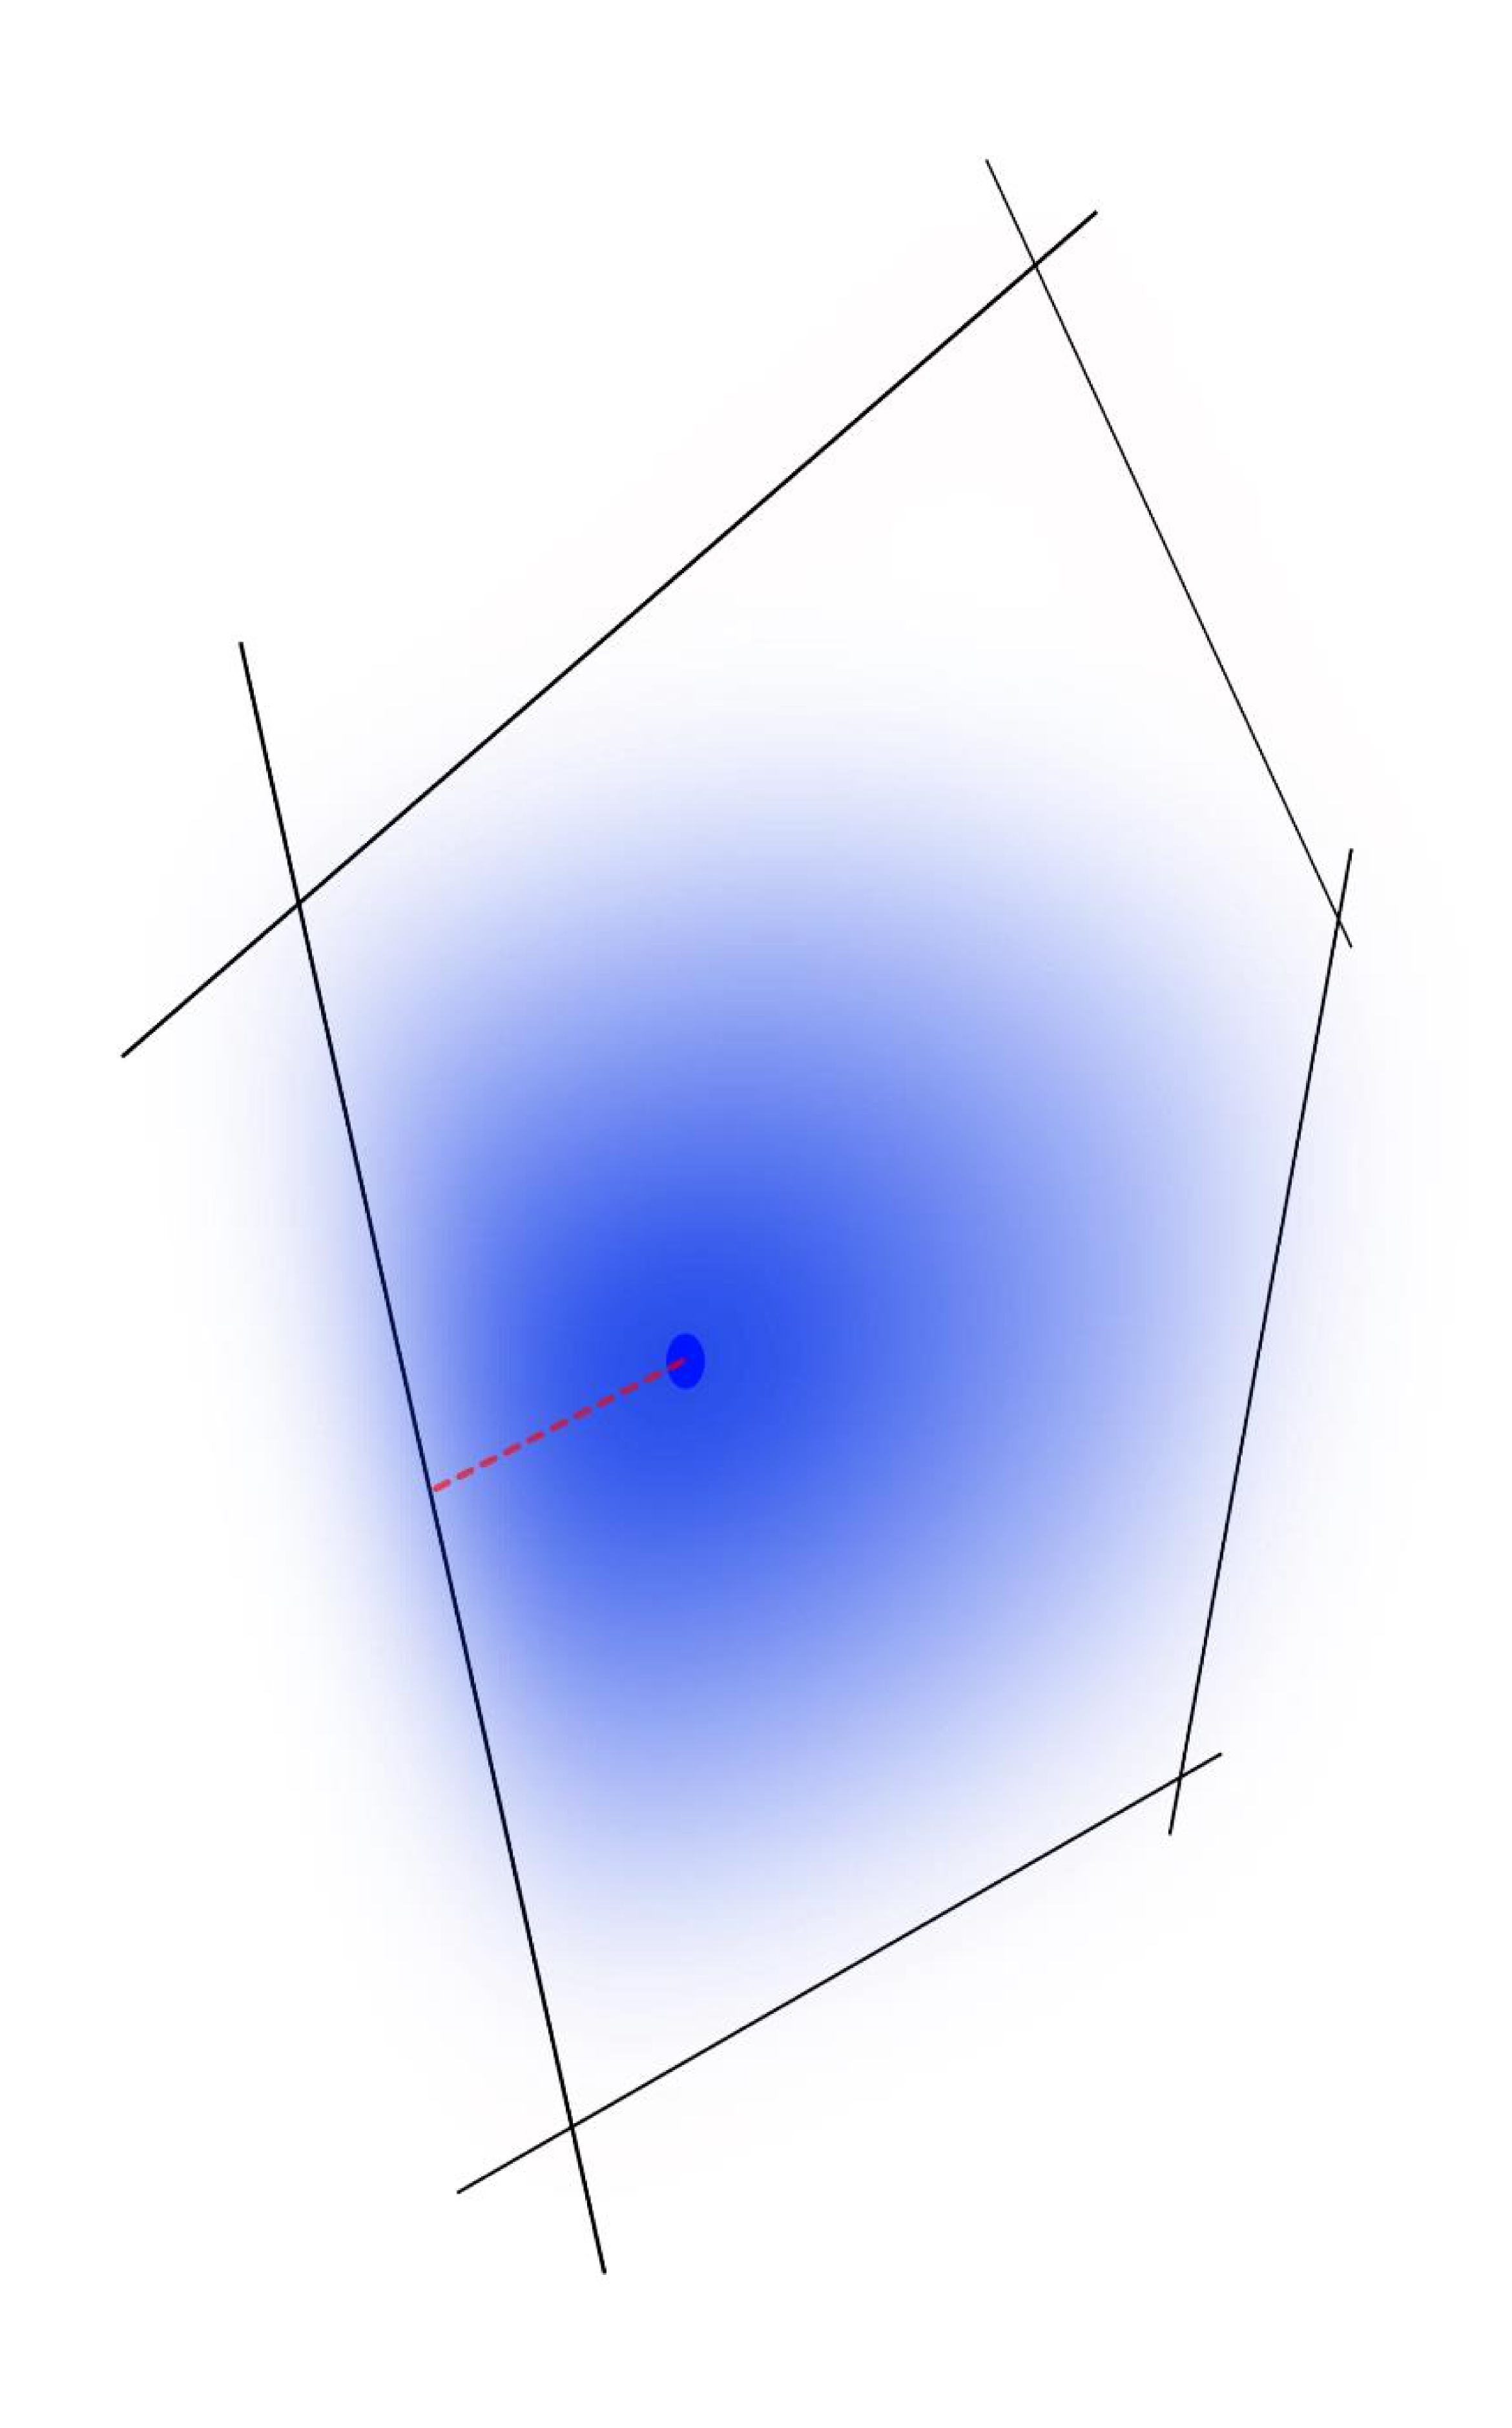
\includegraphics[angle=90,width=0.7\linewidth]{stylizedFeas}
\caption{How far is the forecast operating point from the edge of the feasible region, and might forecast inaccuracies drive the system there?}
\label{fig:stylizedFeas}
\end{figure}

Instanton analysis research falls into two categories. The first is exploration of the trade-off between accuracy and complexity. Replacing the DC power flow approximation with the full AC model, for instance, yields greater accuracy at the cost of convexity \cite{baghsorkhi2012}. Between the DC and AC extremes are various power flow approximations (see \cite{coffrin2012,hijazi2013,coffrin2014} for examples) which may be used to enhance accuracy while maintaining the solution guarantees of convexity. Regardless of the power flow model used, research in this category is ultimately focused on instantaneous vulnerability: find the smallest wind generation shift that drives a line to its steady-state power or current limit. This method uncovers previously hidden grid vulnerability, but may lead to overly-conservative decision making. It is safe to briefly operate a line above its current limit. As long as the line is allowed to cool before sagging to some limit (defined by statute and nearby trees), no harm is done. System operators know this; they periodically allow lines to operate above steady-state limits to promote smooth operation during congestion \cite{banakar2005}. If an operator is comfortable with temporarily overloaded lines, information from instantaneous instanton analysis may be too conservative to aid decision making. Temporal instanton analysis, the second research category, seeks to overcome this limitation by modeling line temperature across multiple time steps.

In this paper we expound on the temporal instanton analysis method introduced in \cite{kersulis2015}. By modeling line temperature over an appropriate time horizon, the proposed method discovers multiple-time-step wind patterns that are both likely to occur and sure to bring at least one line in the network to its temperature limit. The remainder of this paper is organized as follows. Section \ref{sec:models} describes the models at the core of temporal instanton analysis. Section \ref{sec:qcqp} combines these models into a quadratically-constrained quadratic program (QCQP). The solution of this QCQP is described in Section \ref{sec:solution}. Section \ref{sec:implementation}  contains results for two networks: a modified version of the RTS-96 and the larger WECC network. The former network has been used in previous instanton analysis studies, while the latter serves to demonstrate scalability of temporal instanton analysis. Finally, an appendix contains a detailed description of the thermal model used to calculate line temperature.

We expand on prior work by providing a more detailed treatment of the objective function, discussing implementation details including computational complexity and sparsity, and using an improved secular equation solution.

\section{Models}\label{sec:models}
Temporal instanton analysis entwines three physical phenomena. Transmission line temperature is based on a heat balance model, forecast error likelihood is quantified via a statistical model, and the feasible region of network operation is delineated using a network model. This section describes the three models in detail.

\subsection{Transmission Line Heating}\label{sec:models-heat}
A simplified relationship between power flow and line temperature is key to making temporal instanton analysis tractable. Starting with an IEEE standard \cite{ieee2013}, we derive an approximate recursive relationship between a line's temperature at one time step and voltage angle differences at all previous time steps. This relation is summarized below. (Appendix \ref{sec:temp} contains a detailed derivation.)

Consider a time horizon with $n_t$ intervals, each on the order of ten minutes long. Power flow data is updated once per interval (at $t_1,t_2,\ldots,t_{n_t}$), but all other parameters (resistance, solar heating, etc.) remain constant. Choose a single transmission line in the network ---suppose it lies between nodes $i$ and $j$--- and let this line's thermal limit be represented by $T_\text{lim,C}$ ($^\circ$C). We can constrain the line's temperature at time $t_{n_t}$ to be equal to this limiting value by enforcing the constraint
\begin{align}\label{eq:tempconstraint}
\sum_{k=1}^{n_t} \hat{\theta}_{ij}(t_k)^2 &= \frac{a}{c}\left(T_\text{lim,C} - f\right),
\end{align}
where
\begin{subequations}\label{eq:heatbreakdown}
\begin{align}
\label{eq:heatbreakdown-theta}\hat{\theta}_{ij}(t_{k}) &= \theta_{ij}(t_k)\sqrt{ (e^{a\bar{t}})^{n-k+1} - (e^{a\bar{t}})^{n-k} } \\
\label{eq:heatbreakdown-a}a &= \frac{1}{mC_p}\left[ -\eta_c - 4\eta_r T_\text{m,K}^3 \right] \\
\label{eq:heatbreakdown-c}c &= \frac{r_{ij}S_b}{3 mC_p x_{ij}^2L_{ij}} \\
\label{eq:heatbreakdown-d}d &= \frac{ \eta_cT_\text{a,C} + \eta_r\big( 4T_\text{m,C}T_\text{m,K}^3 + T_\text{a,K}^4 - T_\text{m,K}^4   \big) + q_s }{mC_p} \\
\label{eq:heatbreakdown-f}f &= (e^{a\bar{t}})^n T_\text{l,C}^0 + \frac{d}{a}\left[ \sum_{i=1}^n \left( (e^{a\bar{t}})^i - (e^{a\bar{t}})^{i-1} \right)\right]
\end{align}
\end{subequations}

In \eqref{eq:heatbreakdown-theta}, $\theta_{ij}(t_k)$ is the angle difference across line $i-j$ at time interval $t_k$, and $\bar{t}$ is the length of each time interval (e.g. $\bar{t}=t_k-t_{k-1}$). In \eqref{eq:heatbreakdown-a}, $a$ is a constant with units of $s^{-1}$; $mC_p$ is the heat capacity in J/m-$^\circ$C; $\eta_c$ is the conductive heat loss rate coefficient in W/m-$^\circ$C; $\eta_r$ is the conductive heat loss rate coefficient in W/m-$^\circ$C$^4$; and $T_\text{m,K}$ is the average of ambient temperature $T_\text{a,K}$ and limit temperature $T_\text{lim,K}$, in Kelvin. In \eqref{eq:heatbreakdown-c}, $c$ is a constant with units of W/m; $r_{ij}$ and $x_{ij}$ are the resistance and reactance of line $i-j$ in per unit, respectively; $S_b$ is the system base (e.g. 100 MVA); and $L_{ij}$ is the length of one phase of line $i-j$ conductor, in meters. In \eqref{eq:heatbreakdown-d}, $d$ is a constant with units of W/m, and $q_s$ is the solar heat gain rate in W/m. Finally, in \eqref{eq:heatbreakdown-f}, $f$ is a constant with units of degrees Celsius, and $T_\text{l,C}^0 = T_\text{l,C}(t_0)$ is the line's initial temperature (based on generator dispatch and forecast) in Celsius.

\subsection{Wind Forecast Inaccuracy}\label{sec:models-wind}
Distance from the forecast tends to approximate a particular deviation pattern's likelihood,\footnote{For independent power injections like conventional generators or demand nodes, this intuitive model may be adequate.} but spatial and temporal correlation add complexity. Consider several wind farms scattered across a transmission grid, each with a forecast power output. Let the error in this forecast be represented by a zero-mean Gaussian random variable.\footnote{For time scales shorter than roughly one hour, a Cauchy distribution is more appropriate, but forecast errors are commonly assumed to be Gaussian nonetheless. See \cite{hodge2011}.} Then the wind forecast deviation pattern for a single time step takes takes the form of a Gaussian random vector. Elements of this vector are correlated due to spatial relationships between wind sites: if wind speed increases at one site, for instance, a simultaneous decrease at a neighboring site is unlikely. In addition to spatial correlation, there may also be temporal relationships between wind farms.

Suppose a network has $n_r$ wind sites and we wish to consider $n_t$ time intervals. Let $\vec{r}$ be the $(n_t\cdot n_r)\times 1$ vector of forecast deviations across all wind sites and time intervals. The first $n_t$ elements of $\vec{r}$ contain forecast errors for the first site at times $t_1$ to $t_{n_t}$, the second $n_t$ are errors for the second site, and so on. The density function for $\vec{r}$ is
\begin{align}
f(\vec{r}) &= \frac{\exp \left(-\frac{1}{2} \vec{r}^\top \mathbf{C}^{-1} \vec{r} \right)}{(2\pi)^{\frac{n}{2}}\sqrt{\det \mathbf{C}}}~,
\end{align}
where $\mathbf{C}$ is the correlation matrix. Maximizing $f$ corresponds to minimizing $\vec{r}^\top \mathbf{C}^{-1} \vec{r}$. Thus, one may express a desire to maximize wind pattern likelihood with
\begin{align}
\label{eq:obj}\min~ \vec{r}^\top \mathbf{Q} \vec{r},
\end{align}
where $\mathbf{Q}=\mathbf{C}^{-1}$ is the precision matrix. There are many ways to determine $\mathbf{C}$ or $\mathbf{Q}$ from historical data. The authors of \cite{tastu2015} use maximum likelihood optimization to fit a set of parameters to observed data, thereby generating a sparse precision matrix. In our RTS-96 numerical study we assigned reasonable geographic coordinates to each wind site, then mapped distances between site pairs to correlation values using Figure 2.10 of \cite{freris2008}. A third option is to compute a sample correlation matrix from time series data.

\subsection{Network Model}\label{sec:models-network}
Undesirable scenarios found by temporal instanton analysis are of no consequence if they are infeasible. We must therefore restrict our search to the feasible region using power flow constraints. We use a set of linear constraints corresponding to DC power flow with distributed slack.\footnote{DC power flow assumes a flat voltage profile, negligible line resistance (though resistance values are used to calculate line temperatures), and linearity of the sine function.} The mismatch between total power generation and demand at any time step is divided over multiple generators according to participation factors. The next section expresses our power flow model mathematically.

\section{Temporal Instanton QCQP}\label{sec:qcqp}
The following quadratically constrained quadratic program is a concise expression of our desire to find feasible, likely wind patterns that will cause one transmission line in the network to reach its temperature limit by the end of a certain time horizon:
\begin{subequations}\label{eq:opt}
\begin{align}
\label{eq:opt-obj}\underset{\vec{r}}{\min} \quad & \vec{r}^\top \mathbf{Q} \vec{r} \\
\nonumber \text{subject to:} & \\
\label{eq:opt-temp} \sum_{k=1}^{n_t} \hat{\theta}_{ij}(t_k)^2 &= \frac{a}{c}\left(T_\text{lim,C} - f\right)~ \text{for some }(i,j)\in \mathcal{G} \\
\label{eq:opt-flow} \sum_j Y_{ij} \theta_{ij,t_k} & = G_{i,t_k} + (R_{i,t_k} +
\vec{r}_{i,t_k}) - D_{i,t_k} \\[-6pt]
\nonumber &\qquad\qquad\qquad\quad~ \forall i \in 1... n_b,~k\in 1... n_t \\[6pt]
\label{eq:opt-conv} \vec{G}_{t_k} &= \vec{G}_{0,t_k} + \alpha_{t_k}\vec{g} ~~ \forall k\in 1\ldots n_t \\
\label{eq:opt-ref} \theta_{ref,t_k} & = 0 \quad\quad\quad\quad\quad~~ \forall k\in 1\ldots n_t
\end{align}
\end{subequations}
In \eqref{eq:opt}, $n_b$ represents the number of buses (nodes) in the network, $n_t$ the number of time steps, and $\mathcal{G}$ the set of edges (transmission lines). The objective \eqref{eq:opt-obj} matches \eqref{eq:obj} and expresses a desire to find wind patterns that are likely to occur (see Section \ref{sec:models-wind}). In this objective, $\vec{r}$ is the vector of wind output forecast errors, and $\mathbf{Q}$ is the precision (or inverse covariance) matrix. The first constraint \eqref{eq:opt-temp} forces the temperature of a particular line to reach $T_\text{lim,C}$ degrees Celsius at the final time $t_{n_t}$. (See Section \ref{sec:models-heat} for a detailed explanation.) In \eqref{eq:opt-flow}, which enforces DC power balance, $Y_{ij}$ is the $[i,j]$-th element of the admittance matrix (which assumes zero resistance); $\theta_{ij,t_k}$ is the difference between voltage angles $\theta_i$ and $\theta_j$ at time $t_k$; $G_{i,t_k}$ is conventional active power generation at node $i$ and time $t_k$; $(R_{i,t_k} + \vec{r}_{i,t_k})$ is the sum of renewable generation forecast and forecast error for wind node $i$ at time $t_k$ (equal to zero if node $i$ has no wind farm); and $D_{i,t_k}$ is the power demand for bus $i$ at time $t_k$. Constraint \eqref{eq:opt-conv} implements droop response: scheduled generation at time $t_k$ is represented by the vector $G_{0,t_k}$, and each generator $G_i$ compensates for of power mismatch $\alpha_{t_k}$ according to its participation factor $\vec{g}_i$. Finally, the constraint \eqref{eq:opt-ref} establishes the angle reference bus.

The mathematical program \eqref{eq:opt} has a quadratic objective function, a set of linear constraints, and a single quadratic constraint. We can emphasize this QCQP form by combining all variables into a single vector $\mathbf{z}$ and re-writing \eqref{eq:opt} as
\begin{subequations}\label{eq:qcqp}
\begin{align}
\label{eq:qcqp-obj} \min\quad \vec{z}_1^\top &\mathbf{Q}_\text{obj} \vec{z}_1 \\
\label{eq:qcqp-quad}s.t.\quad \vec{z}_3^\top \vec{z}_3 &= c \\
\label{eq:qcqp-lin} \mathbf{A}\vec{z} &= \vec{b}.
\end{align}
\end{subequations}
The objective \eqref{eq:qcqp-obj} is equivalent to \eqref{eq:opt-obj}, the quadratic equality constraint \eqref{eq:qcqp-quad} is equivalent to \eqref{eq:opt-temp}, and the linear equality constraint \eqref{eq:qcqp-lin} combines \eqref{eq:opt-flow}-\eqref{eq:opt-ref}. The vector $\vec{z}$ consists of $n_t\cdot(n_b+n_r+2)$ variables, where $n_t$ is the number of time steps, $n_b$ the number of nodes, and $n_r$ the number of nodes with wind generation. The matrix $\mathbf{A}$ has $n_t\cdot(n_b+2)$ rows: there are $n_b\cdot n_t$ power flow equations \eqref{eq:opt-flow}, $n_t$ equations defining mismatch $\alpha$ at each time step, and $n_t$ auxiliary angle variables defined according to \eqref{eq:heatbreakdown-theta}. Subscripts are used to distinguish variable types: $\vec{z}_1$ contains the $n_t n_r$ wind deviations $\vec{r}$, $\vec{z}_2$ contains the $n_t\cdot(n_b+1)$ angle and mismatch variables, and $\vec{z}_3$ contains the $n_t$ auxiliary angle difference variables involved in line temperature calculation (thereby causing \eqref{eq:qcqp-quad} to take the form of a norm constraint).

Solving \eqref{eq:qcqp} for each line in the network yields a set of instanton candidate wind patterns, each of which will heat a particular line to its thermal limit. Of these candidates, the one with lowest objective value is the instanton wind pattern. The next section contains a solution method for QCQPs of the form \eqref{eq:qcqp}, based in part on work in \cite{bienstock2014}.

\section{QCQP Solution Method}\label{sec:solution}
By now the difference between instantaneous and temporal analyses is clear. Instead of a quadratic program, whose solution readily obtained from KKT conditions, we have a QCQP. The root of this difference is the fact that one cannot express resistive losses---even approximately---as a linear constraint. QCQPs are NP-hard in general; solutions may exist, but unless the quadratic constraint matrices are positive-definite there is no solution guarantee \cite{mehanna2014}. Fortunately, our QCQP belongs to the family of trust region subproblems. As shown in \cite{bienstock2014}, it may be solved in polynomial time. Our solution method, originally presented in \cite{kersulis2015}, divides into four steps.

\subsection{Translation}\label{sec:solution-translation}
The first step is to change variables from $\vec{z}$ to $\vec{y}=\vec{z}-\vec{z}^*$, where
$\vec{z}^* = \arg\min\{\lVert\vec{z}\rVert :\mathbf{A}\vec{z} = \vec{b}\}$. This translation transforms $\mathbf{A}\vec{z} = \vec{b}$ into $\mathbf{A}\vec{y} = \vec{0}$ without qualitatively altering the objective. To
prevent the change from introducing a linear term into the quadratic
constraint, we require $\vec{z}_3^* = \vec{0}$. Thus, we seek the min-norm solution to
\begin{equation}\label{eq:min-norm}
\mathbf{A} \begin{bmatrix} \vec{z}_1^* \\ \vec{z}_2^*
\\ \vec{0} \end{bmatrix} = \vec{b}.
\end{equation}
It is straightforward to find $\vec{z}^*$ by taking the pseudoinverse of $\mathbf{A}$. After translation, the problem becomes
\begin{subequations}\label{eq:translate}
\begin{align}
\label{eq:translate-obj} \min\quad \vec{y}_1^\top &\mathbf{Q}_\text{obj} \vec{y}_1 + 2 \vec{y}_1^\top \mathbf{Q}_\text{obj} \vec{z}_1^* \\
\label{eq:translate-quad} s.t.\quad \vec{y}_3^\top \vec{y}_3 &= c \\
\label{eq:translate-lin} \mathbf{A}\vec{y} &= \vec{0}.
\end{align}
\end{subequations}

\subsection{Kernel mapping}\label{sec:solution-kernel}
The form of \eqref{eq:translate-lin} suggests an intuitive explanation: any solution to \eqref{eq:translate} must lie in the nullspace (kernel) of $\mathbf{A}$. So long as there are no rows of zeros in the matrix of injection shift factors, $\mathbf{A}$ will have full row rank and a $n_t n_r$-dimensional nullspace. We can let $\vec{y}=\mathbf{N}\vec{x}$ where the $n_t n_r$ columns of $\mathbf{N}$ span $\mathcal{N}(\mathbf{A})$. This change of variables is akin to a rotation, but reduces the problem dimension to $n_t n_r$. After partitioning $\mathbf{N}$ so that
\[
\begin{bmatrix} \vec{y}_1 \\ \vec{y}_2 \\ \vec{y}_3 \end{bmatrix} = \begin{bmatrix} \mathbf{N}_1
  \\ \mathbf{N}_2 \\ \mathbf{N}_3 \end{bmatrix} \vec{x},
\]
we can rewrite \eqref{eq:translate} in terms of $\vec{x}$:
\begin{subequations}\label{eq:kernel}
\begin{align}
\label{eq:kernel-obj} \min\quad  &\vec{x}^\top (\mathbf{N}_1^\top \mathbf{Q}_\text{obj}\mathbf{N}_1) \vec{x} + 2\vec{x}^\top
(\mathbf{N}_1^\top \mathbf{Q}_\text{obj} \vec{z}_1^*) \\
\label{eq:kernel-quad} s.t.\quad &\vec{x}^\top \mathbf{N}_3^\top \mathbf{N}_3 \vec{x} = c.
\end{align}
\end{subequations}
All feasible solutions to \eqref{eq:kernel} lie in the nullspace of $\mathbf{A}$, so the linear constraints are now implicit.

\subsection{Obtaining a norm constraint}\label{sec:solution-norm}
After kernel mapping, the quadratic constraint is no longer a norm constraint. This can be corrected by a change of variables. Let $\mathbf{N}_3^\top = \mathbf{USV}^\top$ and $\hat{\mathbf{x}}=\mathbf{U}^\top\mathbf{x}$. The constraint \eqref{eq:kernel-quad} becomes
\begin{equation}
\label{eq:diagonalize} \vec{x}^\top  \mathbf{US}\mathbf
{S}^\top\mathbf{U^\top} \vec{x} = \hat{\mathbf{x}}^\top\mathbf{SS}^\top \hat{\mathbf{x}}=c,
\end{equation}
% First, perform an eigendecomposition $\mathbf{N}_3^\top \mathbf{N}_3 = \mathbf{UDU}^\top$ and let $\hat{\vec{x}} = \mathbf{U}^\top \vec{x}$. The constraint is diagonal in terms of $\hat{\vec{x}}$:
%\begin{equation}
%\label{eq:diagonalize} \vec{x}^\top \mathbf{N}_3^\top \mathbf{N}_3 \vec{x} = \hat{\vec{x}}^\top \mathbf{D}\hat{\vec{x}}
%\end{equation}
where $\mathbf{S}$ is diagonal with at most $n_t$ nonzero elements. The right side of \eqref{eq:diagonalize} may be expanded into
\begin{equation}\label{eq:diagonalize2}
\begin{bmatrix}
\hat{\vec{x}}_1^\top & \hat{\vec{x}}_2^\top \end{bmatrix}
\begin{bmatrix} \hat{\mathbf{S}}^2 & \mathbf{0} \\ \mathbf{0} & \mathbf{0} \end{bmatrix}
\begin{bmatrix}
\hat{\vec{x}}_1 \\ \hat{\vec{x}}_2
\end{bmatrix}.
\end{equation}
The second step is a change of variables from $\hat{\vec{x}}$ to $\vec{w}$ where
\begin{align}
\label{eq:x_to_w} \begin{bmatrix} \vec{w}_1 \\ \vec{w}_2 \end{bmatrix} &=
\begin{bmatrix} \hat{\mathbf{S}} & \mathbf{0} \\ \mathbf{0} & \mathbf{I} \end{bmatrix}
\begin{bmatrix} \hat{\vec{x}}_1 \\ \hat{\vec{x}}_2 \end{bmatrix} = \mathbf{K}\hat{\vec{x}}.
\end{align}
Combine the two steps to relate $\vec{x}$ and $\vec{w}$:
\begin{equation}
\vec{w} = \mathbf{KU}^\top \vec{x}.
\end{equation}
%(Note that $\vec{x} = \mathbf{U}\mathbf{K}^{-1}\vec{w}$ because $\mathbf{UU}^\top = \mathbf{I}$.) In terms of $\vec{w}$, \eqref{eq:kernel-quad} is transformed through \eqref{eq:diagonalize} to give the form of a norm:
%\begin{equation}
%\hat{\vec{x}}^\top \mathbf{D}\hat{\vec{x}} = \hat{\vec{x}}_2^\top \hat{\mathbf{D}}^{1/2}\hat{\mathbf{D}}^{1/2}\hat{\vec{x}}_2
%= \vec{w}_2^\top \vec{w}_2~.
%\end{equation}
In terms of $\vec{w}$, \eqref{eq:kernel} becomes
\begin{subequations}\label{eq:diagonal}
\begin{align}
\label{eq:diagonal-obj} \min\quad &\vec{w}^\top \mathbf{B}\vec{w} + \vec{w}^\top \vec{b} \\
\label{eq:diagonal-quad} s.t.\quad &\vec{w}_1^\top \vec{w}_1 = c,
\end{align}
\end{subequations}
where
\begin{align*}
\mathbf{B} &= \mathbf{K}^{-1}\mathbf{U}^\top \mathbf{N}_1^\top \mathbf{Q}_\text{obj} \mathbf{N}_1 \mathbf{U}\mathbf{K}^{-1} \\
\vec{b} &= 2 \mathbf{K}^{-1}\mathbf{U}^\top
\mathbf{N}_1^\top \mathbf{Q}_\text{obj} \vec{z}_1^*.
\end{align*}
The manipulations in this section have restored the norm structure of the quadratic constraint.

\subsection{Elimination of unconstrained variables}\label{sec:solution-eliminate}
Next we will use the KKT conditions of \eqref{eq:diagonal} to eliminate $\vec{w}_2$, which consists of unconstrained variables. Begin by expanding the objective:
\begin{align*}
f(\vec{w}) &=
\begin{bmatrix} \vec{w}_1^\top & \vec{w}_2^\top \end{bmatrix}
\begin{bmatrix} \mathbf{B}_{11} & \mathbf{B}_{12} \\ \mathbf{B}_{12}^\top & \mathbf{B}_{22}\end{bmatrix}
\begin{bmatrix} \vec{w}_1 \\ \vec{w}_2 \end{bmatrix} +
\begin{bmatrix} \vec{w}_1^\top & \vec{w}_2^\top \end{bmatrix}
\begin{bmatrix} \vec{b}_1 \\ \vec{b}_2\end{bmatrix} \\
&=
\vec{w}_1^\top \mathbf{B}_{11}\vec{w}_1 + 2\vec{w}_1^\top \mathbf{B}_{12}\vec{w}_2 + \vec{w}_2^\top \mathbf{B}_{22}\vec{w}_2 \\
&\qquad + \vec{w}_1^\top \vec{b}_1 + \vec{w}_2^\top \vec{b}_2.
\end{align*}
Next, set the partial derivative with respect to $\vec{w}_2$ equal to zero:
\begin{align}
\nonumber \frac{\partial f}{\partial \vec{w}_2} &= 2\vec{w}_2^\top \mathbf{B}_{22} + 2\vec{w}_1^\top \mathbf{B}_{12} + \vec{b}_2^\top = \vec{0} \\
\label{eq:eliminate} \implies \vec{w}_2 &= -\mathbf{B}_{22}^{-1}\left(\mathbf{B}_{12}^\top\vec{w}_1 +
\frac{1}{2}\vec{b}_2 \right).
\end{align}
After substitution of \eqref{eq:eliminate}, the objective depends only on $\vec{w}_1$:
\begin{align*}
f(\vec{w}_1) &= \vec{w}_1^\top\left(\mathbf{B}_{11} - \mathbf{B}_{12} \mathbf{B}_{22}^{-1}
\mathbf{B}_{12}^\top\right)\vec{w}_1 \\
&\qquad + \vec{w}_1^\top (\vec{b}_1 - \mathbf{B}_{12} \mathbf{B}_{22}^{-1}\vec{b}_2).
\end{align*}
(The constant term, which plays no role in minimization, was omitted.) Thus, \eqref{eq:diagonal} is equivalent to a $n_t$-dimensional program with a single norm constraint:
\begin{subequations}\label{eq:eliminated}
\begin{align}
\min\quad & \vec{w}_1^\top \hat{\mathbf{B}}\vec{w}_1 - 2\vec{w}_1^\top \hat{\vec{b}} \\
\label{eq:eliminated-quad} s.t.\quad & \vec{w}_1^\top \vec{w}_1 = c,
\end{align}
\end{subequations}
where
\begin{align*}
\hat{\mathbf{B}} &= \mathbf{B}_{11} - \mathbf{B}_{12} \mathbf{B}_{22}^{-1}
\mathbf{B}_{12}^\top \\
\hat{\vec{b}} &= -\frac{1}{2}\left(\vec{b}_1 - \mathbf{B}_{12} \mathbf{B}_{22}^{-1}\vec{b}_2\right).
\end{align*}

\subsection{Solution via iteration}\label{sec:solution-enumeration}
A straightforward method of solving \eqref{eq:eliminated} involves initially diagonalizing $\hat{\mathbf{B}}$ (by the process described in Section \ref{sec:solution-norm}). Now let $v$ be the Lagrange multiplier associated with the constraint \eqref{eq:eliminated-quad}, and write the first-order optimality conditions:
\begin{subequations}\label{eq:first-order}
\begin{align}
\label{eq:kkt} \hat{\mathbf{B}}\vec{w}_1 &= v\vec{w}_1~ + \hat{\vec{b}} \\
\mathbf{w}_1^\top \mathbf{w}_1 &= c
\end{align}
\end{subequations}
This system is equivalent to the \textit{secular equation}
\begin{align*}
f(v) &= \sum_{i=1}^n \left(\frac{\hat{\mathbf{b}}_i}{\hat{\mathbf{B}}_{i,i}-v}\right)^2 - c,
\end{align*}
which has between 2 and $2n_t$ solutions.\footnote{This is apparent from the graph of a secular equation. See \cite{gander1989}.} Obtaining all solutions would require traversing the curve from each pole (nonzero diagonal element of $\hat{\mathbf{B}}$) in both directions. Fortunately, the proof in Appendix \ref{sec:lagrange} shows that optimizing \eqref{eq:eliminated} is equivalent to minimizing $v$ subject to \eqref{eq:first-order}. Because $\mathbf{w}_1^\top \mathbf{w}_1$ is a monotonically increasing function of $v$ from $-\infty$ to the smallest nonzero diagonal element of $\hat{\mathbf{B}}$, we can obtain the smallest feasible value of $v$ using the following iterative relationship (due to \cite{gander1989}):
\begin{align*}
v^{(i+1)} &= v^{(i)} - 2\frac{f\left(v^{(i)}\right) + c}{f'\left(v^{(i)}\right)}\sqrt{\frac{f\left(v^{(i)}\right) + c}{c}} - 1.
\end{align*}
The value of $v$ obtained at convergence corresponds to the optimal $\mathbf{w}_1$ in \eqref{eq:eliminated}. Reversing all variable changes yields the optimal value for $\mathbf{z}$ in the original solution space. This vector specifies wind site active power deviations, voltage angles, and the active power mismatch at each time step.

Each line in the network has its own QCQP and solution vector $\mathbf{z}$. Once each line's QCQP has been solved, the set of solution vectors may be sorted by objective value \eqref{eq:qcqp-obj}. Lines whose solutions have small objective value are more likely to reach unacceptable temperatures due to changes in wind; lines with large objective value are comparatively robust to wind fluctuations. The vector $\mathbf{z}$ with lowest objective is the \textit{instanton}.

\section{Implementation}\label{sec:implementation}
We focus on implementation details in two areas: pre-analysis checks to rule out infeasible QCQPs, and numerical considerations that determine overall computational requirements and scaling.

\subsection{Pre-analysis checks}
Pre-analysis checks can identify two situations that lead to infeasible temporal instanton QCQPs. First, if a line's resistance is zero, it must be excluded.\footnote{Of course, zero-resistance lines are more an artifact of network bookkeeping than a physical reality.} Equation \eqref{eq:lossapprox} indicates power loss will be zero for such lines regardless of flow, so wind variations have no effect on their temperature. The second check makes use of injection shift factors. Suppose a network's topology and wind site placement is such that power flow for a particular line is completely unaffected by changes in wind generation. In this scenario, line temperature is isolated from changes in decision variables, and our QCQP is infeasible. Fortunately, DC injection shift factors may be used to skip such lines: whenever a line's flow is detached from changes in wind, its shift factors with respect to all wind nodes will be zero. 
%\begin{figure}[!t]
%\centering
%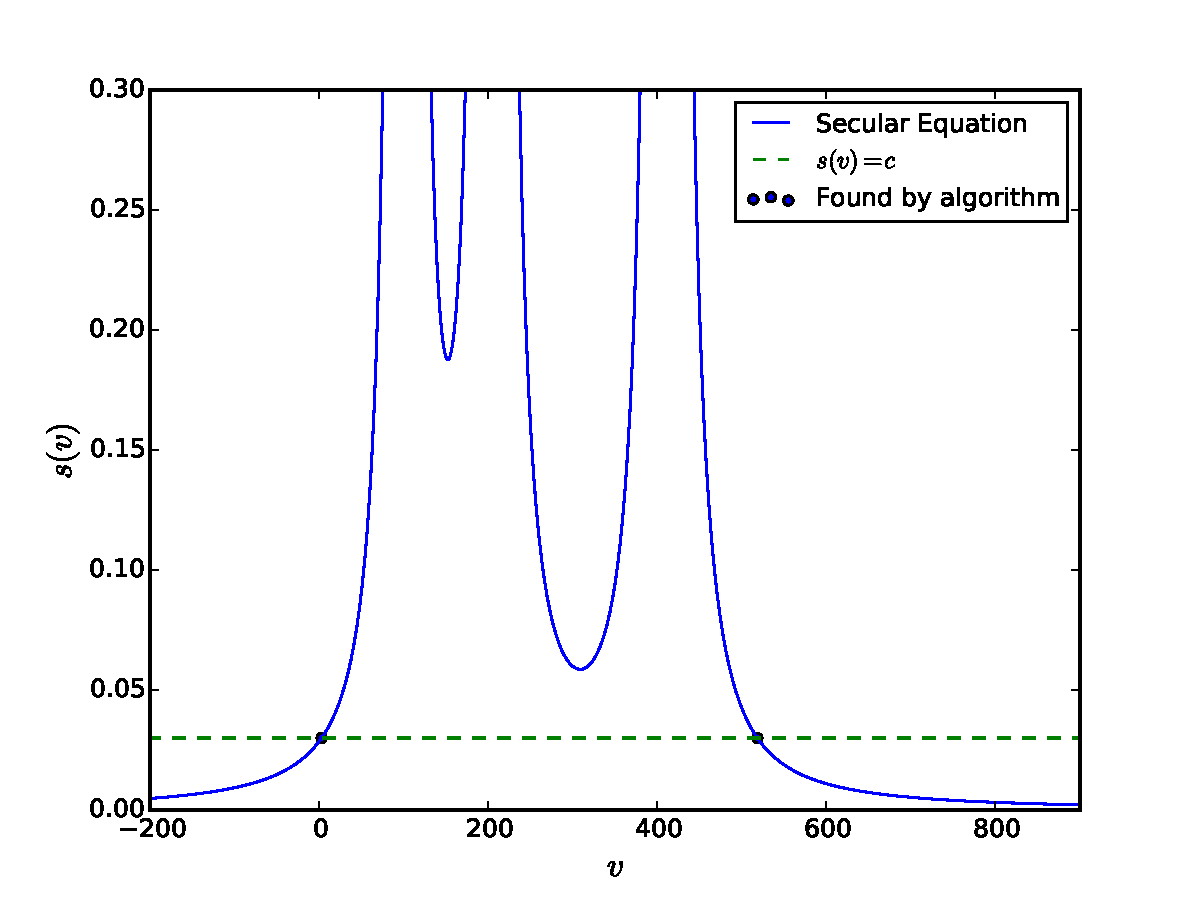
\includegraphics[trim=0.3in 0.in 0.7in 0.4in,clip,width=1\linewidth]{secular}
%\caption{Secular equation for a single line (corresponding to the instanton) in the RTS-96. Because there were six time steps in the analysis, $s(v)$ approaches infinity at six poles. Dots show the six solutions to $s(v) = c$ identified by our secular equation solver. Note that there could be as few as two solutions if $c$ were small enough.}
%\label{fig:secular}
%\end{figure}

\subsection{Computational burden and algorithm scaling}
Temporal instanton analysis consists of solving a Section \ref{sec:qcqp} QCQP via the Section \ref{sec:solution} method for each line in the network. Each QCQP is independent from, and nearly identical to, all others.\footnote{Only the $n_t$ rows of $\mathbf{A}$ corresponding to auxiliary angle variables $\hat{\theta}$ change as one line is replaced by another.} This pleasing parallelism means total processing time grows linearly with the number of lines analyzed. In the remainder of this section we focus on individual QCQPs.
%Provided one has as many computing cores as there are lines in the network, solution time may be reduced to that of a single QCQP (plus overhead for initialization, memory sharing, and aggregation of results). 
Solution time for a single QCQP varies with network size, wind site placement, and algorithm design.
%\footnote{The relationship between number of workers and overall performance may not be intuitive. On our four-core laptop, two workers were able to cut overall computation time in half with a modest increase in memory allocation. When we used four worker processes, however, the savings were eclipsed by communication and data sharing costs.}
%Computation and storage requirements for a single QCQP vary with network size, wind site placement, and factorization methods used.
Reasoning from algorithmic complexity and numerical results, we call attention to considerations that characterize scaling.

%\subsection{Sparsity}\label{sec:implementation-sparsity}
Sparsity is of the utmost importance in numerical implementation of temporal instanton analysis. Because each piece of \eqref{eq:qcqp} is dominated by zeros, sparsity plays a key role in storage requirements before manipulations even begin. The objective, for example, contains only a subset $\vec{z}_1$ of the variables; portions of $\mathbf{Q}_\text{obj}$ corresponding to $\vec{z}_2$ and $\vec{z}_3$ consist entirely of zeros. Even the nonzero portion of $\mathbf{Q}_\text{obj}$ (the precision matrix $\mathbf{Q}$) is sparse if the method of \cite{tastu2015} is used to generate it. The constraints \eqref{eq:qcqp-quad} and \eqref{eq:qcqp-lin} are similarly sparse: a dense representation of \eqref{eq:qcqp-quad} for the RTS-96 network with six time steps occupies 2.5 megabytes; a sparse version takes just 40 bytes. The benefits of sparsity carry through to concatenation, multiplication, and factorization.

%\subsection{Factorization}\label{sec:implementation-factorization}
Matrix factorization, a relatively expensive operation, plays a significant role in determining overall algorithm scaling. Three factorizations are required in the Section \ref{sec:solution} solution method. First, a portion of the $\mathbf{A}$ matrix must be factorized to find its pseudoinverse and determine the min-norm translation point $\vec{z}^*$ in \eqref{eq:min-norm}. A sparse Cholesky factorization is appropriate here. A second factorization is necessary to construct a basis for the kernel of $\mathbf{A}$. Here one might use a sparse QR factorization or, if the $\mathbf{A}$ matrix is well-conditioned, an LU-based approach to save time.\footnote{The SPQR algorithm in SuiteSparse \cite{foster2011} is well suited for the QR-based approach. The LU approach involves column operations on the $\mathbf{A}$ matrix augmented with identity below. If QR factorization is used, this step takes more than a third of total computation time.}
%the "one-third" figure is only valid for the RTS-96. may not scale that way to other scenarios.
Another necessary factorization is the singular value decomposition required for diagonalizing the constraint (see Section \ref{sec:solution-norm}). Because $\mathbf{N}_3$ is $n_rn_t$-by-$n_t$, it has only $n_t$ nonzero singular values. These may be found directly using a dense SVD algorithm, but it is more efficient to retrive them via Arnoldi iteration.\footnote{An appropriate algorithm is described in \cite{lehoucq1996} and implemented in ARPACK. It is available in MATLAB, SciPy, and Julia environments through the \texttt{eigs} and \texttt{svds} functions.} The fourth factorization is less demanding: block LU decomposition may be used to inexpensively expose the Schur complements needed to compute $\hat{\mathbf{B}}$ and $\hat{\mathbf{b}}$ in \eqref{eq:eliminated}; see \cite{zhang2006}.

%\subsection{Algorithm Scaling}
We performed two tests to characterize scaling of our algorithm. First, we varied the number of wind nodes (and, therefore, decision variables) in the RTS-96 network and, considering a time horizon of one hour divided into six ten-minute intervals, performed a complete analysis in each case. Figure \ref{fig:rts-96-scaling} illustrates the relationship between QCQP size and the average QCQP solution time. Second, we added wind farms to ten of the test cases packaged with MATPOWER \cite{zimmerman2011} and analyzed each. For each network we replaced a fixed portion of conventional generation with wind, placed wind sites randomly, and sized each site to fix overall wind penetration to $70\%$. The choice of these parameters is somewhat arbitrary for the purposes of characterizing algorithm scaling, but we were careful to add enough significantly-sized wind farms to each network to avoid numerical difficulties.\footnote{If there are too few wind nodes or penetration is too low, many solutions will have absurdly high objective value.} Figure \ref{fig:normalized-performance} shows average computation time for a single QCQP versus network size. As a reference point for overall solution time, it took just over two hours for our four-core laptop with 8 GB of RAM to analyze every line in the Polish summer 2008 peak network (case \texttt{3120sp} in Matpower). The same analysis applied to the RTS-96 network takes roughly half a second.
% this time has decreased significantly; note the new time in the final version.

%Our numerical experimentation raises new questions. What is the relationship between the number of wind farms (decision variables) and algorithm performance? How does the solution time of a single QCQP vary with network size and topology?

\begin{figure}[!t]
\centering
\includegraphics[trim=0in 0in 0in 0.38in,clip,width=1.05\linewidth]{rts-96-scaling-dots-2}
\caption{Average computation time per QCQP solution versus number of decision variables. The network is the 73-node RTS-96, and the time horizon is one hour divided into six ten-minute intervals. Starting with two, the number of wind farms is increased two at a time up to 72, and these wind farms are randomly placed throughout the network. The ratio of forecast wind generation to conventional generation is fixed at 0.7. Analysis was repeated thirty times to illustrate the effects of wind farm placement on solution times; light gray lines indicate average QCQP solution times for individual trials.}
\label{fig:rts-96-scaling}
\end{figure}

\begin{figure}[!t]
\centering
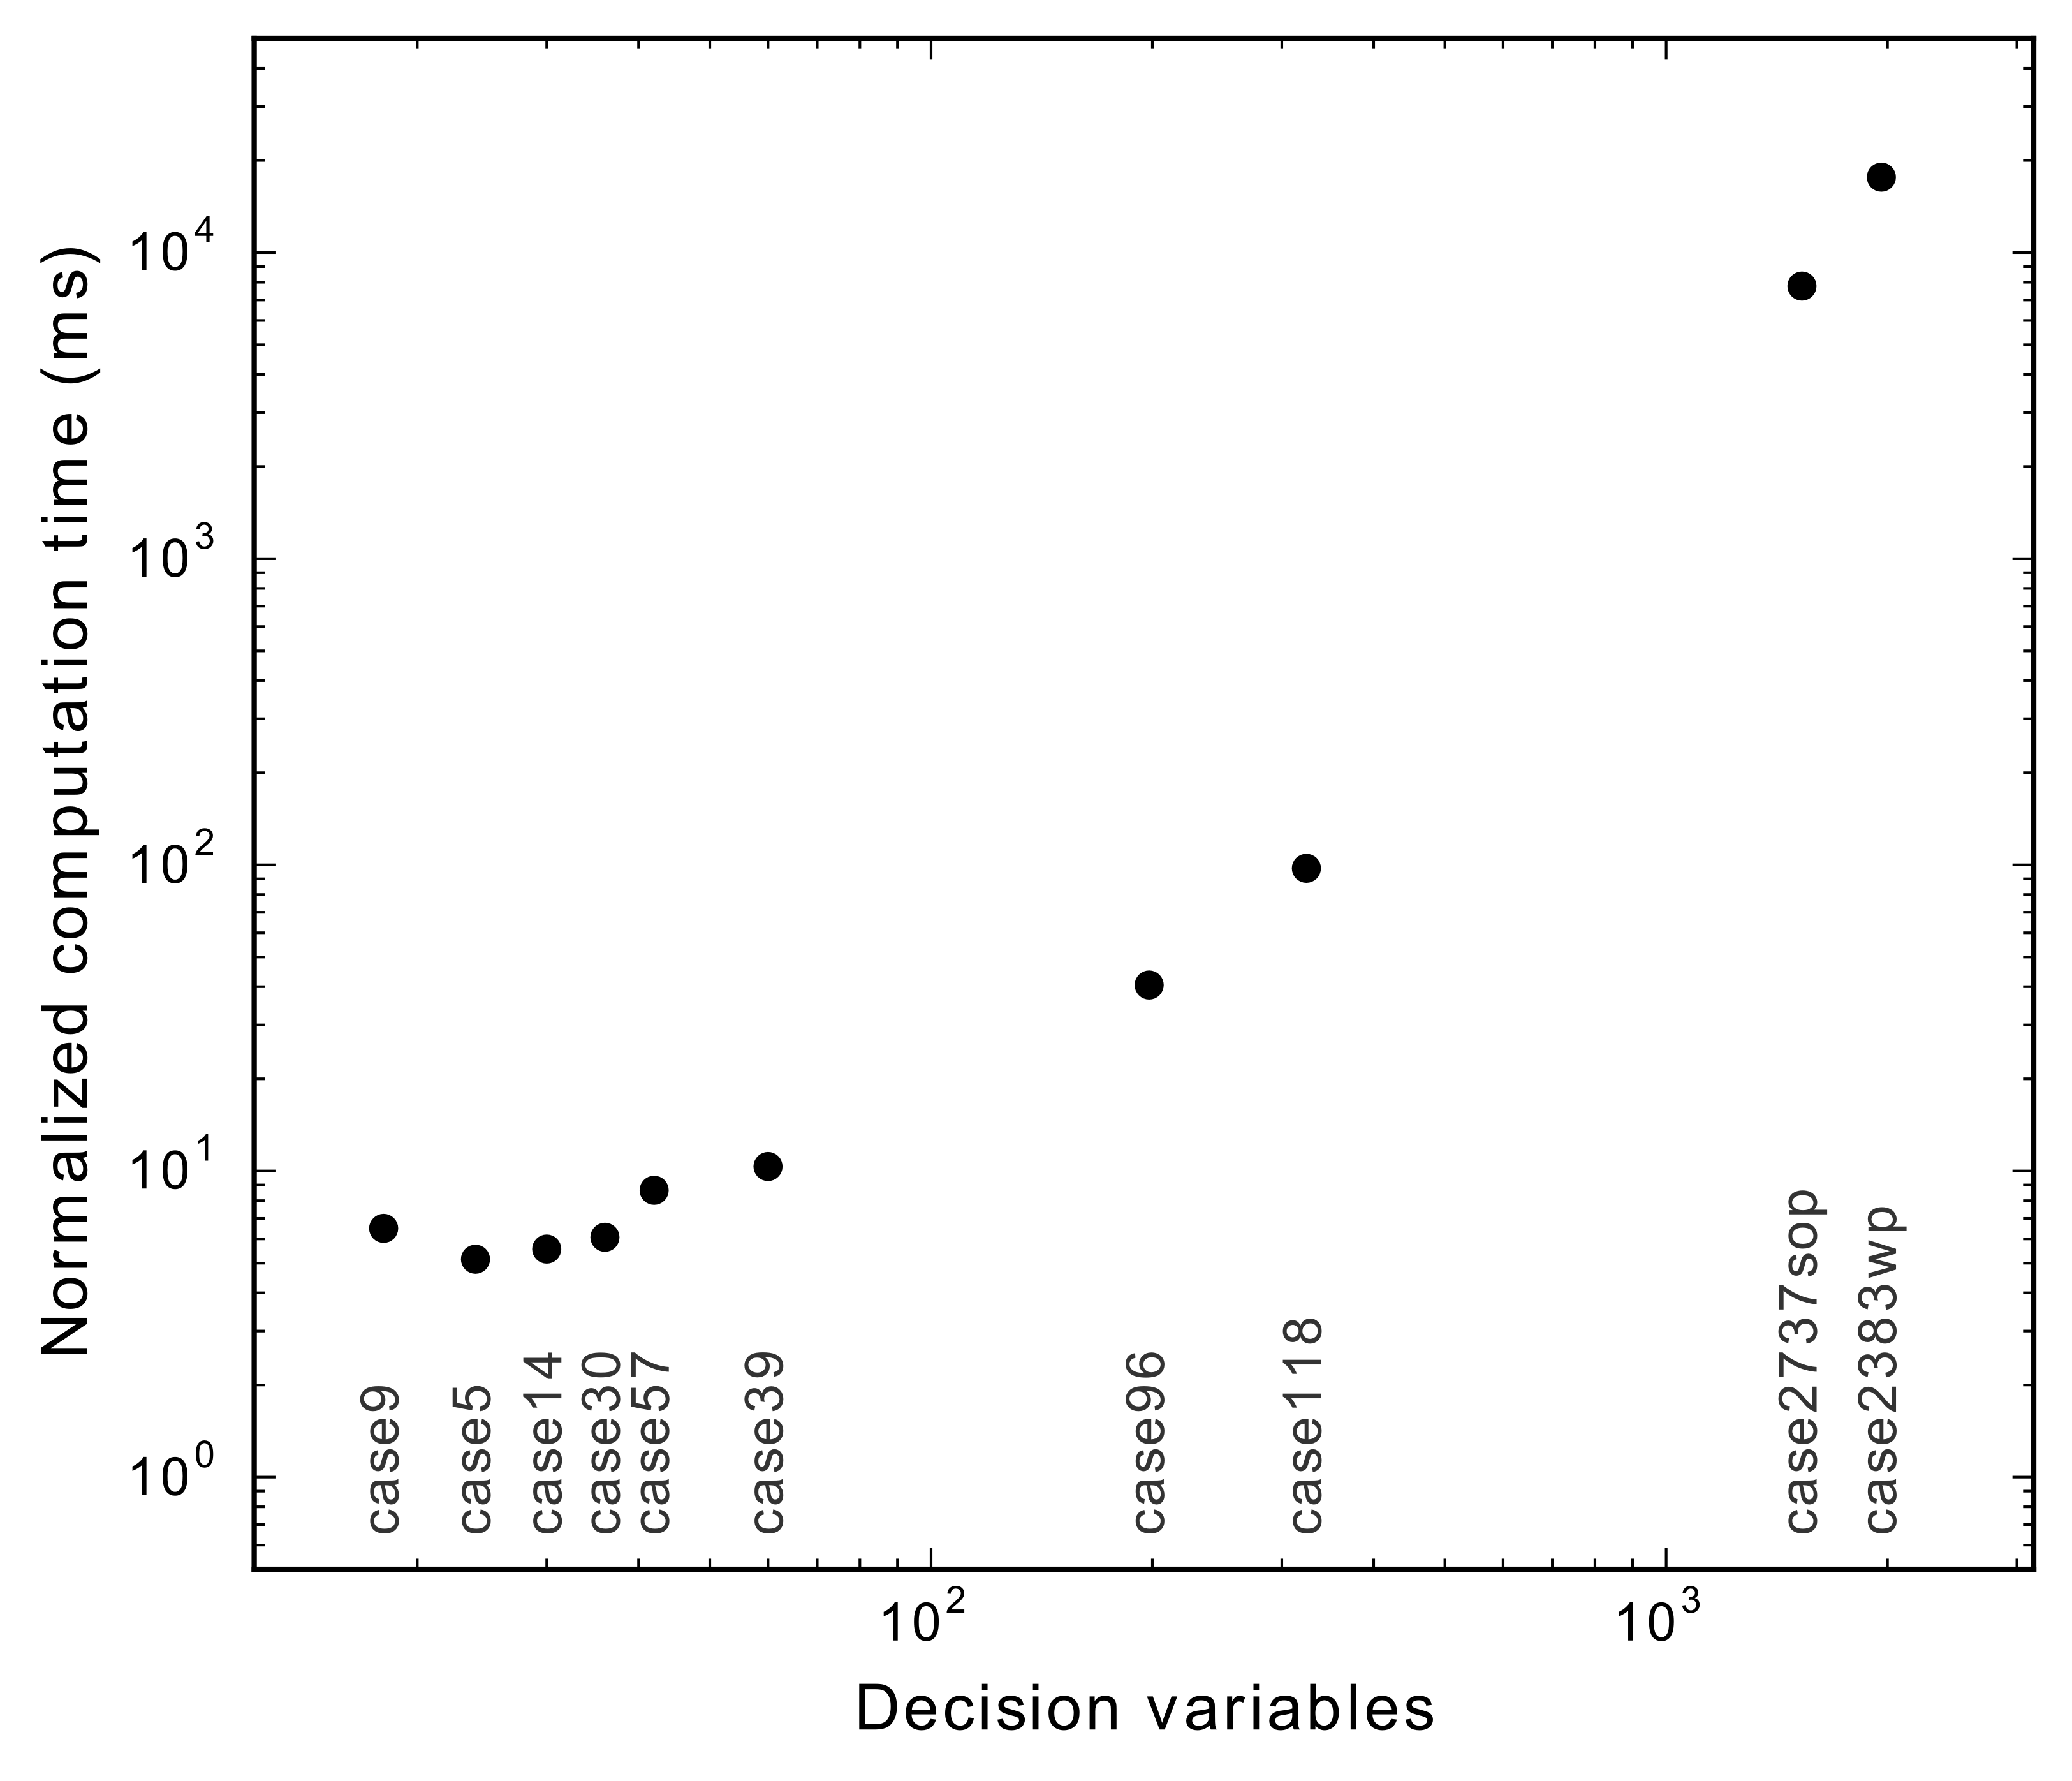
\includegraphics[trim=0in 0in 0in 0in,clip,width=0.95\linewidth]{normalized-performance}
\caption{Average computation time (total time divided by number of lines analyzed) for ten Matpower cases, on a log-log scale. For each network, the number of wind farms is equal to the number of conventional generators, and wind nodes were chosen randomly. In every case the time horizon is five minutes divided into six thirty-second intervals.}
\label{fig:normalized-performance}
\end{figure}

\section{Results}\label{sec:results}
Numerical results are included for two purposes. The first is to illustrate the relationship between the instanton pattern and a line's temperature trajectory. How does line temperature evolve in response to instanton angle differences? Second, numerical experimentation can illustrate the effects of wind covariance. What impact does a reasonable covariance matrix have on instanton objective values and wind patterns? In each experiment we used the modified RTS-96 network from \cite{pandzic}, assumed Waxwing conductors as in \cite{almassalkhi2015}, considered six time steps, and gradually increased the wind forecast over time while keeping conventional generation and demand constant.

\subsection{Temperature Trajectories}
%Our modified RTS-96 network has eighteen wind farms distributed across three areas: nine in the first area, six in the second, and three in the third.
We assume all lines begin at $60^\circ$C and have temperature limits of $65^\circ$C. We performed instanton analysis for a one-hour time horizon divided into six ten-minute intervals. Figure \ref{fig:temptrajectory} illustrates temperature trajectories corresponding to the instanton and nearby wind patterns. The instanton pattern causes the line to reach $65^\circ$C, but if we randomly perturb the vector of forecast deviations while keeping its norm (objective value) constant, the line does not reach its temperature limit. This illustrates that the solution found by our algorithm is the most likely wind forecast deviation pattern with respect to the wind model described in Section \ref{sec:models-wind}.

\begin{figure}[!t]
\centering
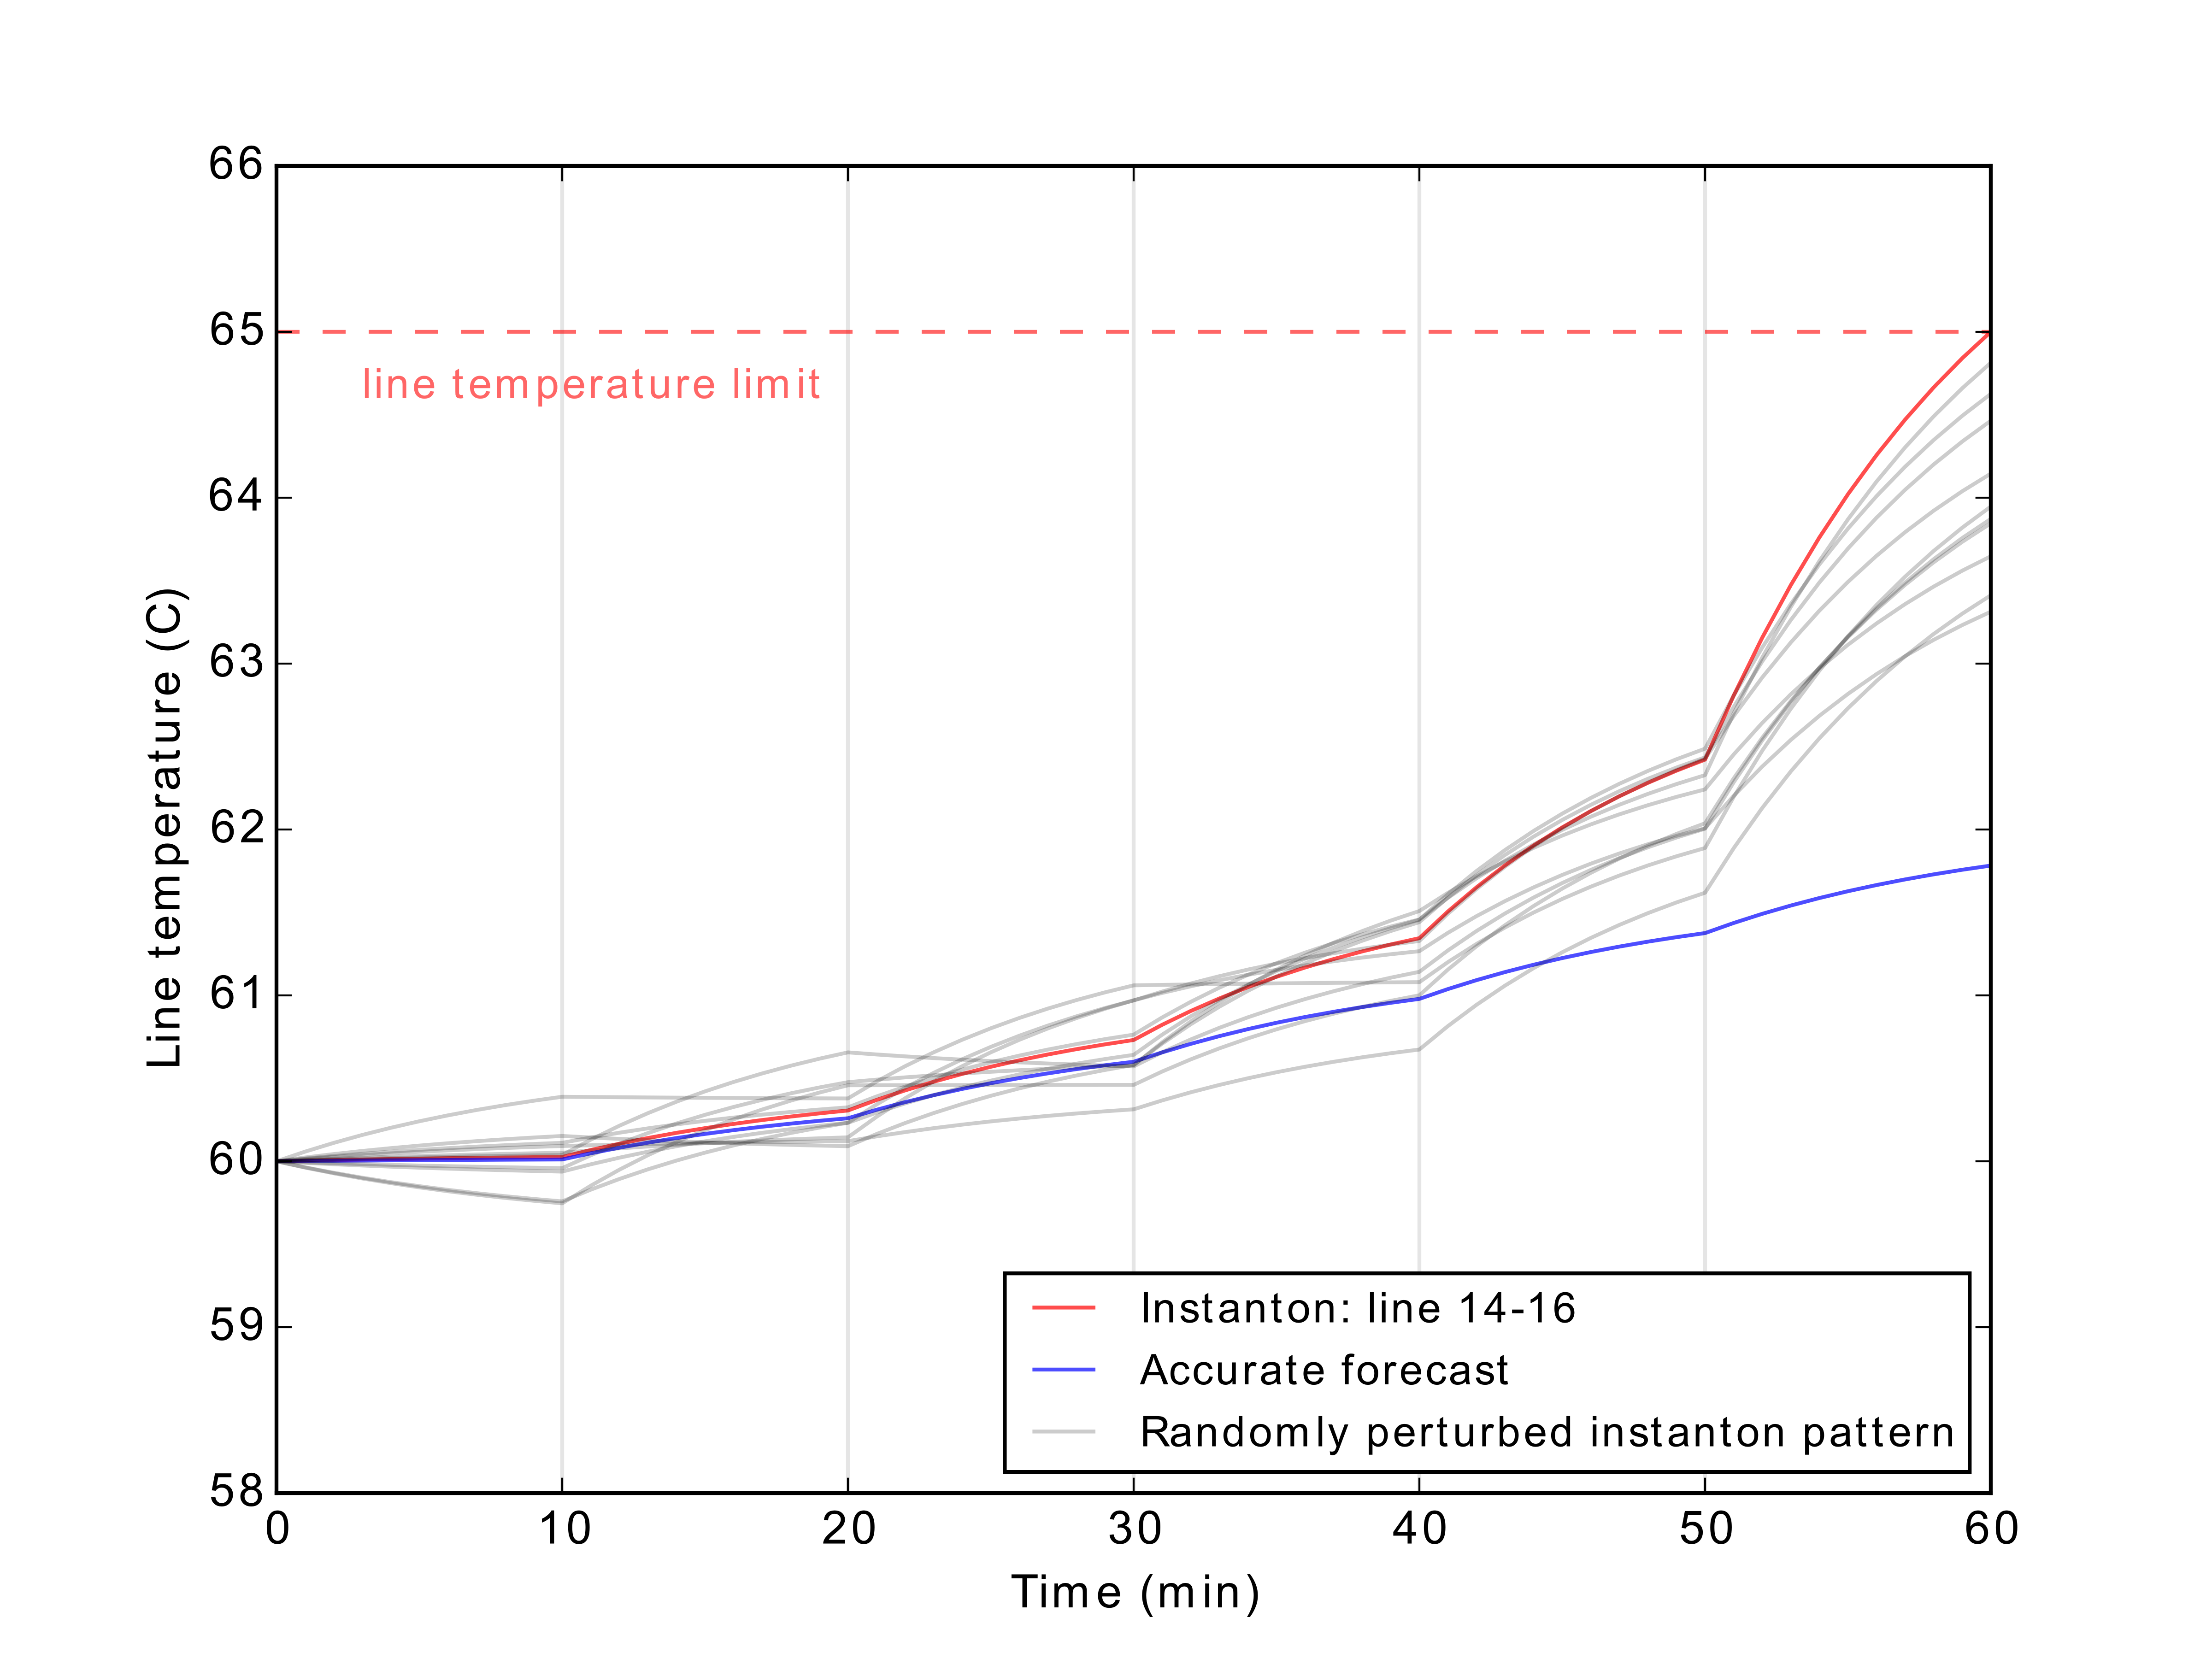
\includegraphics[trim=0.3in 0.in 0.7in 0.5in,clip,width=0.9\linewidth]{temptrajectory}
\caption{RTS-96 temperature trajectories for the line between nodes 14 and 16. Red represents the instanton trajectory, which brings the line to its temperature limit of 65 C. Trajectories shown in gray arise from randomly perturbed versions of the instanton wind pattern having the same objective value. The blue trajectory corresponds to zero deviation from the wind forecast.}
\label{fig:temptrajectory}
\end{figure}

\subsection{Effects of Covariance}
To illustrate the effects of covariance on temporal instanton analysis, we used a simple heuristic method to generate a reasonable spatial covariance matrix for the RTS-96. After assigning geographic coordinates to each of the eighteen wind farms and constructing a distance matrix, we mapped distances to correlation coefficients using a relationship from \cite{freris2008}. This positive-definite, unit-norm covariance matrix weights wind deviations at all time steps, allowing the QCQP solution algorithm to find patterns with lower objective value by increasing highly correlated deviations. Figure \ref{fig:covariance} shows that these patterns have higher objective value when the original objective function (simple two-norm) is used.

\begin{figure}[!t]
\centering
\includegraphics[trim=0.3in 0.in 0.7in 0.4in,clip,width=0.95\linewidth]{covariance}
\caption{Objective values for lowest forty instanton candidates, with and without covariance. ``Covariance output measured by norm objective'' was computed by passing solution vectors from the covariance analysis output to the objective function from the no-covariance case.}
\label{fig:covariance}
\end{figure}

\section{Conclusion}\label{sec:conclusion}
This paper has extended the temporal instanton analysis method presented in \cite{kersulis2015} with a focus on implementation and algorithm scaling. Models for each of the three phenomena involved in temporal instanton analysis were presented
%: changes in transmission line temperature were related to voltage angle differences via a DC line loss approximation, wind forecast error likelihood was represented by the weighted two-norm of a vector of forecast deviation variables, and power balance and generator droop response were modeled with a standard DC power flow linear system. The three models were
and combined into a QCQP, and a solution algorithm was presented. Important numerical considerations were then discussed, and algorithm scaling was illustrated. Finally, numerical results were presented to show temperature trajectories and the effects of wind covariance.
%Although computational demands scale in a predictable fashion, the results themselves depend on many factors. These include the number, size, and placement of wind farms; network parameters including line conductor type, line length, and impedance; and ambient conditions like solar radiation.
%Of particular interest is the effect of wind farm placement on instanton candidate objective scores. If wind farms are concentrated in one portion of the grid, for example, some lines may have instanton candidates with low objective value while other lines have no solutions at all. This may be interpreted in terms of injection shift factors: some nodes have greater influence on a particular line's flow than others. Though shift factors provide intuition for some solution behavior, the complex web of parameters involved in temporal instanton analysis calls for analysis and interpretation in future work.

% Note that IEEE typically puts floats only at the top, even when this
% results in a large percentage of a column being occupied by floats.

\appendices
\section{Line Temperature Model}\label{sec:temp}

%\subsection{Heat Balance Equation}
The change in temperature of any object may be expressed as a differential equation called the heat balance equation, which relates temperature change to a sum of various sources of heating. The IEEE 738 standard \cite{ieee2013} provides the following heat balance equation for a transmission line:

\begin{align}\label{eq:heatbalance}
\frac{dT}{dt} &= \frac{1}{m\cdot C_p}\left[I^2\cdot R(T_\text{l,C}(t)) - q_c - q_r + q_s \right]
\end{align}
In \eqref{eq:heatbalance}, $T_\text{l,C}(t)$ is the conductor average temperature in Celsius, $m\cdot C_p$ is the product of mass and heat capacity, and $I^2\cdot R(T_\text{l,C}(t))$ represents heat rate due to resistive heating. $q_c$ represents convective heat loss, which is proportional to the temperature difference between the line and surrounding air:
\begin{align}\label{eq:qc}
q_c &= \eta_c\cdot(T_\text{l,C}(t) - T_\text{a,C})~,
\end{align}
where $T_\text{a,C}$ is the ambient temperature in Celsius. $q_r$ in \eqref{eq:heatbalance} represents radiation heat loss, modeled by the fourth-order expression
\begin{align}\label{eq:qr}
 q_r &= \eta_r\cdot\left[T_\text{l,K}(t)^4 - T_\text{a,K}^4\right],
\end{align}
where $T_\text{l,K}(t)$ and $T_\text{a,K}$ are the conductor and ambient temperatures in Kelvin, respectively. Finally, $q_s$ in \eqref{eq:heatbalance} represents solar heating. In this paper $q_s$ is fixed to some conservative constant (corresponding to full, direct sun).

%\subsection{DC Line Loss Approximation}
We replace the resistive heat rate term $I^2\cdot R(T_\text{l,C}(t))$ by $f_{ij}^\text{loss}$, the approximate line loss expression derived in \cite{almassalkhi2014}:
\begin{equation}\label{eq:lossapprox}
f_{ij}^{\text{loss}} \approx r_{ij}\left(\frac{\theta_{ij}}{x_{ij}}\right)^2,
\end{equation}
where $\theta_{ij}$ is the difference between angles $\theta_i$ and $\theta_k$, and $r_{ij} +j x_{ij}$ is the impedance of the line between nodes $i$ and $j$. Three DC power flow assumptions underpin \eqref{eq:lossapprox}: voltage magnitudes are all 1pu, cosine may be approximated by its second-order Taylor expansion, and $x_{ij} \geq 4r_{ij}$. Thus, \eqref{eq:lossapprox} provides an approximates line losses using voltage angle differences.

%\subsection{Linearization of Radiation Heat Rate}
When \eqref{eq:heatbalance} is combined with an initial temperature $T_\text{l,C}^0$ and \eqref{eq:lossapprox}, the resulting initial value problem should make it possible to determine conductor temperature $T_\text{l,C}(t_n)$ at a later time $t_n$. We substitute \eqref{eq:qc}-\eqref{eq:lossapprox} into \eqref{eq:heatbalance} and attempt to solve for temperature:
\begin{multline}\label{eq:heatbalance_approx}
\frac{dT}{dt} = \frac{1}{mC_p}\big[ f_{ij}^\text{loss} - \eta_c\left( T_\text{l,C}(t) - T_\text{a,C}\right) \\ - \eta_r\left(T_\text{l,K}(t)^4 - T_\text{a,K}^4\right) + q_s \big]
\end{multline}
If power flow, ambient temperature, and solar heat rate are constant, this differential equation is still fourth-order in conductor temperature $T_\text{C}(t)$ due to radiation. Fortunately, $q_r$ is approximately linear over our temperature range of interest (from ambient temperature to temperature limit). We replace $q_r$ by the conservative linearization\footnote{Because a transmission line is hotter than surrounding air, radiation tends to decrease line temperature. Thus, a conservative approach will underestimate $q_r$. Plotting \eqref{eq:approx_rad} shows that it does indeed underestimate $q_r$.}
\begin{align}\label{eq:approx_rad}
\tilde{q}_r &= \eta_r  \left( T_\text{m,K}^4 - T_\text{a,K}^4\right) +  4\eta_rT_\text{m,K}^3(T_\text{l,C}(t) - T_\text{m,C}),
\end{align}
where $T_\text{m,C}$ is the average (midpoint between) ambient and conductor limit temperatures in Celsius, and $T_\text{m,K}$ is $T_\text{m,C}$ converted to Kelvin. After substitution of \eqref{eq:approx_rad}, the heat balance equation becomes linear in conductor temperature, and the IVP has a straightforward solution.

%\subsection{Line Temperature as Recursive Relationship}
Substitution of \eqref{eq:approx_rad} into \eqref{eq:heatbalance_approx} yields the approximate heat balance equation
\begin{align}\label{eq:diffeq}
\frac{dT_\text{l,C}}{dt} &= aT_\text{l,C}(t) + b~,
\end{align}
where constants $a$ and $b$ are defined as
\begin{subequations}
\begin{align}
a &= \frac{1}{mC_p} \left[ -\eta_c - 4\eta_rT_\text{m,K}^3 \right]
\end{align}
\begin{multline}
b = \frac{1}{mC_p} \big[ f_{ij}^\text{loss} + \eta_cT_\text{a,C} - \eta_r \left( T_\text{m,K}^4 - T_\text{a,K}^4 \right) \\ + 4\eta_rT_\text{m,C}\cdot T_\text{m,K}^3 + q_s \big]
\end{multline}
\end{subequations}

The IVP \eqref{eq:diffeq} has a straightforward solution:
\begin{align}\label{eq:tivp}
T_\text{l,C}(t) &= ke^{at} - \frac{b}{a},
\end{align}
where $k=T_\text{l,C}(0) + b/a$. Note that $b$ is influenced by power flow (via
$f_{ij}^\text{loss}$ according to \eqref{eq:lossapprox}), but $a$ is not. The only variables in \eqref{eq:tivp} are initial temperature and angle differences during each time interval. There is therefore a recursive relationship between final temperature and initial temperature that involves only angle differences. The derivation of this recursive relationship is an exercise in messy linear algebra; it is omitted here for brevity. The final relationship is expressed in \eqref{eq:tempconstraint}, where it is used as a line temperature constraint.

%\newcommand{\splitcell}[2][c]{%
%\begin{tabular}[#1]{@{}c@{}}#2\end{tabular}}
%\begin{table}
%\begin{center}
%\caption{Line heating parameters}
%\label{tab:heatparams}
%\begin{tabular}{|c|c|c|}
%	\hline
%	         Parameter           &   Units    &               Description                \\ \hline
%	           $T_s$             &    $s$     &               Sample time                \\ \hline
%	           $mC_p$            & $J/(m\cdot C)$ & \splitcell{Per-unit-length heat capacity\\of the conductor}         \\ \hline
%	          $\eta_c$           & $W/(m\cdot C)$ &     \splitcell{Conductive heat loss \\ rate coefficient}         \\ \hline
%	          $\eta_r$           & $W/(m\cdot C)$ &      \splitcell{Radiative heat loss\\rate coefficient}         \\ \hline
%	       $T^\text{lim}$        &    $C$     &      \splitcell{Line temperature at\\steady-state current limit.}   \\ \hline
%	       $\Delta q_{s,ij}$ & $W/m$ & \splitcell{Solar heat input\\ into conductor} \\ \hline
%	       $\Delta T_\text{amb}$ & C & \splitcell{Change in \\ambient temperature} \\ \hline
%\end{tabular}
%\end{center}
%\end{table}

\section{Lagrange Multiplier Proof}\label{sec:lagrange}
\subsection{Statement}
The following two optimization problems are equivalent:
\begin{subequations}
\begin{align}
\nonumber &(P) &\min~ & \mathbf{w}^\top \hat{\mathbf{B}} \mathbf{w} - 2\hat{\mathbf{b}}^\top \mathbf{w} & \\
\nonumber & s.t. & \mathbf{w}^\top \mathbf{w} &= c \\ 
\nonumber &(P') & \min~ & u  \\
\label{eq:Pprime-kkt}& s.t.& \mathbf{w}^\top \mathbf{w} &= c \\
\label{eq:Pprime-norm}&& \hat{\mathbf{B}}\mathbf{w} &= u \mathbf{w} + \hat{\mathbf{b}}~.
\end{align}
\end{subequations}
(Note that $\hat{\mathbf{B}}$ is diagonal, and $(P)$ is equivalent to \eqref{eq:eliminated}.)

\subsection{Proof}
It is sufficient to prove that if $(u_1,\mathbf{w}_1)$ and $(u_2,\mathbf{w}_2)$ satisfy the first-order conditions \eqref{eq:Pprime-kkt}-\eqref{eq:Pprime-norm} with $u_1 < u_2$, then
\begin{align*}
f(\mathbf{w}_1) = \mathbf{w}_1^\top \hat{\mathbf{B}} \mathbf{w}_1 - 2\hat{\mathbf{b}}^\top \mathbf{w}_1 &< \mathbf{w}_2^\top \hat{\mathbf{B}} \mathbf{w}_2 - 2\hat{\mathbf{b}}^\top \mathbf{w}_2 = f(\mathbf{w}_2).
\end{align*}
We proceed using a technique from \cite{gander1989}. By \eqref{eq:Pprime-kkt} we have:
\begin{subequations}
\begin{align}
\label{eq:first3} \hat{\mathbf{B}}\mathbf{w}_1 &= u_1 \mathbf{w}_1 + \hat{\mathbf{b}} \\
\label{eq:first4} \hat{\mathbf{B}}\mathbf{w}_2 &= u_2 \mathbf{w}_2 + \hat{\mathbf{b}}
\end{align}
\end{subequations}
Multiply both \eqref{eq:first3} and \eqref{eq:first4} by $\mathbf{w}_1^\top$ and $\mathbf{w}_2^\top$ to obtain
\begin{subequations}
\begin{align}
\label{eq:2a}\mathbf{w}_1^\top \hat{\mathbf{B}} \mathbf{w}_1 &= u_1 c + \mathbf{w}_1^\top \hat{\mathbf{b}} \\
\label{eq:2b}\mathbf{w}_2^\top \hat{\mathbf{B}} \mathbf{w}_2 &= u_2 c + \mathbf{w}_2^\top \hat{\mathbf{b}} \\
\label{eq:2c}\mathbf{w}_1^\top \hat{\mathbf{B}} \mathbf{w}_2 &= u_2\mathbf{w}_1^\top \mathbf{w}_2 + \hat{\mathbf{b}}^\top \mathbf{w}_1 \\
\label{eq:2d}\mathbf{w}_2^\top \hat{\mathbf{B}} \mathbf{w}_1 &= u_1\mathbf{w}_2^\top \mathbf{w}_1 + \hat{\mathbf{b}}^\top \mathbf{w}_2,
\end{align}
\end{subequations}
where \eqref{eq:Pprime-norm} was used to replace instances of $\mathbf{w}_1^\top \mathbf{w}_1$ and $\mathbf{w}_2^\top \mathbf{w}_2$ with $c$. Now subtract \eqref{eq:2b} from \eqref{eq:2a} to obtain
\begin{align*}
(\mathbf{w}_1^\top \hat{\mathbf{B}} \mathbf{w}_1 - \mathbf{w}_1^\top \hat{\mathbf{b}}) - (\mathbf{w}_2^\top \hat{\mathbf{B}} \mathbf{w}_2 - \mathbf{w}_2^\top \hat{\mathbf{b}}) &= (u_1 - u_2)c.
\end{align*}
Add $\hat{\mathbf{b}}^\top \mathbf{w}_2$ and subtract $\hat{\mathbf{b}}^\top \mathbf{w}_1$ to yield
\begin{align*}
f(\mathbf{w}_1) - f(\mathbf{w}_2) &= (u_1 - u_2)c - \mathbf{w}_1^\top \hat{\mathbf{b}} + \mathbf{w}_2^\top \hat{\mathbf{b}},
\end{align*}
then substitute \eqref{eq:2c} and \eqref{eq:2d}:
\begin{align*}
f(\mathbf{w}_1) - f(\mathbf{w}_2) &= (u_1 - u_2)c + (u_2 - u_1) \mathbf{w}_1^\top \mathbf{w}_2 \\
&=  (u_1 - u_2)(c - \mathbf{w}_1^\top \mathbf{w}_2)
\end{align*}
Note that $\lVert \mathbf{w}_1 - \mathbf{w}_2 \rVert = \mathbf{w}_1^\top \mathbf{w}_1 + \mathbf{w}_2^\top \mathbf{w}_2 - 2\mathbf{w}_1^\top \mathbf{w}_2 = 2c - 2\mathbf{w}_1^\top \mathbf{w}_2$, so
\begin{align*}
f(\mathbf{w}_1) - f(\mathbf{w}_2) &= \frac{1}{2}(u_1 - u_2)\lVert \mathbf{w}_1 - \mathbf{w}_2 \rVert.
\end{align*}
Because $u_1 < u_2$, the right-hand size is negative. The objective value corresponding to $\mathbf{w}_1$ is therefore less than that of $\mathbf{w}_2$. We conclude that $(P)$ and $(P')$ are equivalent.

%\section*{Acknowledgment}
%The authors would like to thank Dr. M. Chertkov and Dr. S. Backhaus of Los Alamos National Laboratory for discussions and notes that assisted in the transition from instantaneous to temporal settings, and Dr. D. Bienstock for his expertise and practical assistance in the solution of trust region subproblems. We also thank David Hiskens and Dr. R. Nadakuditi at the University of Michigan for helpful discussion and references related to secular equation solutions.

% Can use something like this to put references on a page
% by themselves when using endfloat and the captionsoff option.
%\ifCLASSOPTIONcaptionsoff
%  \newpage
%\fi

% trigger a \newpage just before the given reference
% number - used to balance the columns on the last page
% adjust value as needed - may need to be readjusted if
% the document is modified later
%\IEEEtriggeratref{8}
% The "triggered" command can be changed if desired:
%\IEEEtriggercmd{\enlargethispage{-5in}}

% references section

\bibliographystyle{IEEEtran}
\bibliography{bib}

\newpage

%\begin{IEEEbiography}{Jonas Kersulis}
%(S'12) received the B.S. degree in electrical engineering from the University of Missouri-St. Louis, St. Louis, MO USA; and the M.S. degree in Electrical Engineering:Systems from the University of Michigan, Ann Arbor, MI, USA, where he is currently working on his PhD.
%
%His research interests include power system modeling and optimization.
%
%Jonas is a member of the IEEE Power and Energy Society.
%\end{IEEEbiography}
%
%\begin{IEEEbiography}{Ian A. Hiskens}
%(S'77--M'80--SM'96--F'06) received the B.Eng. degree in electrical engineering and the B.App.Sc. degree in mathematics from the Capricornia Institute of Advanced Education, Rockhampton, Australia, in 1980 and 1983 respectively, and the Ph.D. degree in electrical engineering from the University of Newcastle, Australia, in 1991.
%
%He is the Vennema Professor of Engineering
%in the Department of Electrical Engineering and Computer Science, University of Michigan, Ann Arbor, MI, USA. He has held prior appointments in the Queensland electricity supply industry, and various universities in Australia and the United States. His research interests lie at the intersection of power system analysis and systems theory, with recent activity focused largely on integration of renewable generation and controllable loads.
%
%Dr. Hiskens is actively involved in various IEEE societies, and is VP-Finance of the IEEE Systems Council. He is a Fellow of Engineers Australia, and a Chartered Professional Engineer in Australia.
%\end{IEEEbiography}


% if you will not have a photo at all:
%\begin{IEEEbiographynophoto}{John Doe}
%Biography text here.
%\end{IEEEbiographynophoto}

% insert where needed to balance the two columns on the last page with
% biographies
%\newpage

%\begin{IEEEbiographynophoto}{Jane Doe}
%Biography text here.
%\end{IEEEbiographynophoto}

% You can push biographies down or up by placing
% a \vfill before or after them. The appropriate
% use of \vfill depends on what kind of text is
% on the last page and whether or not the columns
% are being equalized.

%\vfill

% Can be used to pull up biographies so that the bottom of the last one
% is flush with the other column.
%\enlargethispage{-5in}

\end{document}


